\documentclass[conference]{IEEEtran}

\usepackage{cite}
\usepackage{amsmath,amssymb}
\usepackage{graphicx}
\usepackage{booktabs}
\usepackage{tikz}
\usepackage{xcolor}
\usepackage{hyperref}
\usepackage{pgfplots}
\pgfplotsset{compat=newest}

\hypersetup{
    colorlinks=true,
    linkcolor=blue,
    citecolor=blue,
    urlcolor=blue
}

\begin{document}

\title{Historical Case Study on Ti Silicide (TiSi\textsubscript{2}) \\
Reliability Issues in Mixed-Voltage CMOS Driver ICs}

\author{
\IEEEauthorblockN{Shinichi Samizo}
\IEEEauthorblockA{Independent Semiconductor Researcher\\
Project Design Hub, Samizo-AITL\\
\textit{Email:} \href{mailto:shin3t72@gmail.com}{shin3t72@gmail.com}\quad
\textit{GitHub:} \href{https://github.com/Samizo-AITL}{Samizo-AITL}}
}

\maketitle

\begin{abstract}
This paper analyzes a historical case from the early 2000s in LCD driver IC development.  
Although the 0.18~µm CMOS process was already available and stable, manufacturers adopted the 0.25~µm LOCOS-based process to enable reliable integration of 30~V high-voltage devices.  
However, the use of Ti silicide (TiSi\textsubscript{2}) in the 0.25~µm node introduced instability due to incomplete C49$\rightarrow$C54 transformation and boron absorption, leading to random bit failures in 1~Mbit SRAM macros.  
This case illustrates the trade-offs between memory scaling, process stability, and device isolation technology.
\end{abstract}

\section{Introduction}
In the late 1990s, LCD driver ICs for monochrome passive-matrix panels dominated, typically fabricated using 0.35~µm processes supporting 3.3~V logic and 40~V high-voltage devices.  
With the transition to color active-matrix (aTFT) panels in the early 2000s, driver ICs required higher-performance logic, embedded large SRAM macros, and continued high-voltage integration.  

At this time, 0.18~µm CMOS was in production, but it used Shallow Trench Isolation (STI), where edge thinning created risks for 30~V device integration.  
In contrast, the 0.25~µm process still employed Local Oxidation of Silicon (LOCOS), which had proven reliability for high-voltage devices.  
Therefore, manufacturers chose the 0.25~µm LOCOS-based process for mixed 3.3~V + 30~V integration.

\section{Technical Background}
\subsection{LOCOS vs. STI for High-Voltage Devices}
\begin{itemize}
  \item \textbf{0.25~µm LOCOS}: supported 30~V device integration, with proven isolation margin.
  \item \textbf{0.18~µm STI}: process-stable but required new high-voltage development due to isolation thinning.
\end{itemize}

\begin{table}[!t]
\centering
\caption{Comparison of 0.25~µm LOCOS vs. 0.18~µm STI Processes}
\begin{tabular}{@{}lll@{}}
\toprule
 & 0.25~µm LOCOS & 0.18~µm STI \\
\midrule
Isolation & LOCOS, HV proven & STI, edge thinning risk \\
HV device mix & 30~V feasible & new 30~V dev. needed \\
SRAM capacity & up to 1~Mbit & more compact, lower area \\
Stability & silicide instabilities & stable process baseline \\
\bottomrule
\end{tabular}
\end{table}

\subsection{Ti Silicide Issues}
TiSi\textsubscript{2} was adopted for low resistivity but required a C49$\rightarrow$C54 phase transformation.  
Incomplete transition left high-resistance C49 grains.  
Additionally, boron absorption from halo implants aggravated resistivity variation.  
While 500~kbit SRAM macros had been in production without major issues, the scaling to 1~Mbit exposed these latent instabilities.

\section{Failure Case: 1Mbit SRAM}
\subsection{Observation}
In mass production, random single-bit failures appeared in the 1~Mbit SRAM macro.  
Since redundancy was not implemented in the macro, even one defective bit caused chip rejection.

\subsection{Root Cause}
Failure localization confirmed that:
\begin{itemize}
  \item Halo boron was absorbed into Ti during salicide formation.
  \item This inhibited C54 formation locally, leaving high-resistive C49 regions.
  \item These spots manifested as random SRAM cell failures.
\end{itemize}

\subsection{Review Limitation}
Earlier products with 500~kbit SRAM macros had not revealed this issue, leading engineers to assume 1~Mbit scaling would be acceptable.  
Thus, the failure mode was not captured at design review.

\section{Countermeasures}
\subsection{Provisional}
Etch profiles were tuned to undercut sidewalls, increasing separation between halo regions and Ti, which improved yield significantly.

\subsection{Permanent}
RTA conditions were optimized to favor stable C54 formation.  
However, this altered device parameters and required re-characterization.

\section{Yield Sensitivity Model}
The yield impact of redundancy can be approximated by a Poisson model:
\[
Y_k = e^{-\lambda} \sum_{i=0}^{k} \frac{\lambda^i}{i!},
\]
where $\lambda$ is the average defect count, and $k$ is the redundancy capacity.

\begin{figure}[!t]
  \centering
  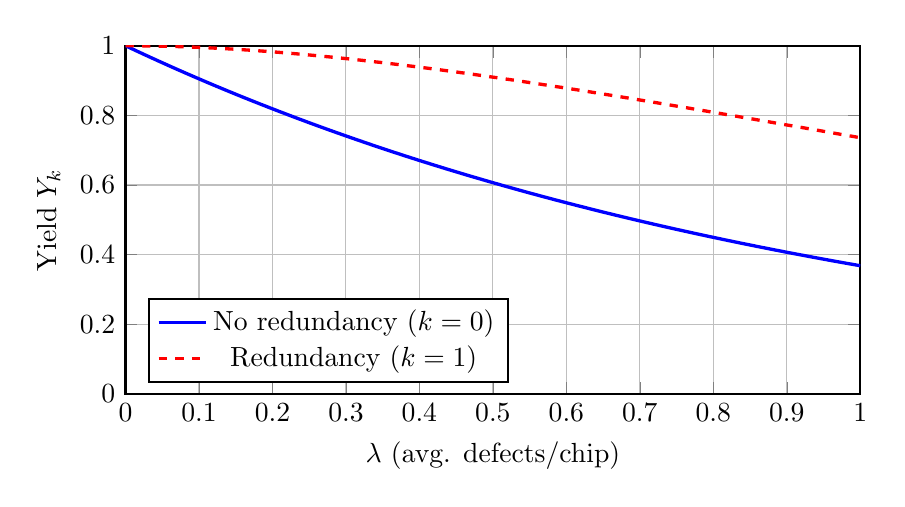
\begin{tikzpicture}
    \begin{axis}[
      width=0.9\linewidth,
      height=6cm,
      xlabel={$\lambda$ (avg. defects/chip)},
      ylabel={Yield $Y_k$},
      xmin=0, xmax=1,
      ymin=0, ymax=1,
      legend pos=south west,
      grid=both,
      thick,
    ]
      \addplot[blue, very thick, domain=0:1, samples=200] {exp(-x)};
      \addlegendentry{No redundancy ($k=0$)}

      \addplot[red, dashed, very thick, domain=0:1, samples=200] {exp(-x)*(1+x)};
      \addlegendentry{Redundancy ($k=1$)}
    \end{axis}
  \end{tikzpicture}
  \caption{Yield sensitivity with and without redundancy (Poisson model).}
  \label{fig:yield}
\end{figure}

\section{Educational Application}
\subsection{Teaching Tools}
\begin{itemize}
  \item Cause-effect diagram: process $\rightarrow$ defect $\rightarrow$ yield
  \item Comparative table: LOCOS (0.25~µm) vs. STI (0.18~µm)
  \item Exercise: process improvement vs. redundancy adoption
\end{itemize}

\subsection{Lessons}
The critical point was reliance on 500~kbit SRAM yield data to justify 1~Mbit macros.  
Combined with Ti silicide instability, this created a failure mode unseen in earlier products.  
Since STI processes were not yet reliable for 30~V integration, 0.25~µm LOCOS was the only feasible choice.

\section{Conclusion}
This case shows how:
\begin{itemize}
  \item LOCOS enabled 30~V device integration, driving the adoption of 0.25~µm even after 0.18~µm was available.
  \item Ti silicide instability, invisible at 500~kbit, became critical at 1~Mbit SRAM scale.
  \item Design reviews relying solely on prior yield experience failed to anticipate this.
\end{itemize}
The educational value lies in recognizing how scaling, process technology, and high-voltage requirements intersect in semiconductor history.

\section*{References}
\begin{thebibliography}{99}
\bibitem{Sze2007} S. M. Sze and K. K. Ng, \textit{Physics of Semiconductor Devices}, 3rd ed. Wiley, 2007.
\bibitem{Wolf1986} S. Wolf and R. N. Tauber, \textit{Silicon Processing for the VLSI Era, Vol. 1: Process Technology}. Lattice Press, 1986.
\bibitem{Colinge2004} J.-P. Colinge, \textit{Silicon-on-Insulator Technology: Materials to VLSI}, 3rd ed. Springer, 2004.
\bibitem{ITRS2001} International Technology Roadmap for Semiconductors (ITRS), ``Process Integration, Devices, and Structures,'' 2001.
\bibitem{Takeda1994} E. Takeda, C. Y. Yang, and A. S. Grove, ``Silicide technology for ULSI applications,'' \textit{IEEE Trans. Electron Devices}, vol. 41, no. 12, pp. 2133--2141, Dec. 1994.
\bibitem{Chang1996} J. P. Chang and A. J. Steckl, ``Titanium silicide formation and stability in submicron CMOS technology,'' \textit{J. Appl. Phys.}, vol. 79, no. 9, pp. 4536--4364, 1996.
\end{thebibliography}

\section*{Author Biography}
\textbf{Shinichi Samizo} received the M.S. degree in Electrical and Electronic Engineering from Shinshu University, Japan.  
He worked at Seiko Epson Corporation on semiconductor memory and mixed-signal device development and contributed to inkjet MEMS actuators and PrecisionCore printhead technology.  
He is currently an independent semiconductor researcher focusing on process/device education, memory architecture, and AI system integration.\\
\emph{Contact:} \href{mailto:shin3t72@gmail.com}{shin3t72@gmail.com}\quad
\emph{GitHub:} \href{https://github.com/Samizo-AITL}{Samizo-AITL}.

\end{document}
